% Dokumentenklasse (festgelegt!)
\documentclass{llncs}

% Allgemeine Einstellungen
\usepackage[utf8]{inputenc} % Zeichenkodierung auf UTF8
\usepackage[ngerman]{babel} % Deutsche Anpassungen, z.B. Trennregeln
\usepackage[T1]{fontenc} % T1-Zeichenkodierung einschalten, damit z.B. Umlaute im PDF-Dokument gesucht werden können

\usepackage[a4paper,top=3cm,bottom=2cm,left=3cm,right=3cm,marginparwidth=1.75cm]{geometry}

% Quellenverzeichnis:
\usepackage[backend=biber, style=numeric, sorting=none]{biblatex}
\addbibresource{Seminar_Quellenverzeichnis.bib}

% für TODO Kommentare:
\usepackage{todonotes}

% Quellcode-Abbildungen:
\usepackage{listings}

% Vektorgrafiken
\usepackage{svg}

% Tabellenbeschriftung
\usepackage{caption}
\captionsetup[table]{position=below,skip=1em}

% Farbe in Tabellenzellen:
\usepackage{colortbl}
\definecolor{hellgrau}{rgb}{0.95,0.95,0.95} % Farbdefinition, kann im Code verwendet werden

% Bilder einbinden:
\usepackage{graphics}
\graphicspath{{./img/}} % Angabe von Ordner für Bilder
\usepackage{subcaption}


\begin{document}
\title{Intertask Kommunikation in Echtzeitbetriebsystemen}
\author{Stefan Lindörfer\\
\email{stefan.lindoerfer@stud-mail.uni-wuerzburg.de}
}
\institute{
	Universität Würzburg\\
	Institut für Informatik\\
	Lehrstuhl V - Technische Informatik\\
	Seminar: Embedded Systems\\Prof. Dr. Reiner Kolla\\Wintersemester 2020/21}

%\date{}

\maketitle

\renewcommand{\abstractname}{Abstract}

\begin{abstract}
	Die Informationsübermittlung zwischen Tasks in Echtzeitbetriebsystemen ist von fundamentaler Bedeutung und kann je nach Anforderungsszenario auf verschiedene Arten erfolgen. In der vorliegenden Arbeit wird zunächst ein Überblick über die verschiedenen Möglichkeiten gegeben sowie darauffolgend jeweils vertieft auf die Mechaniken eingegangen und durch Beispiele demonstriert.
\end{abstract}

\section{Einführung}
\label{subsec:Einführung}
Echtzeitbetriebsysteme (auch \textbf{R}eal \textbf{T}ime \textbf{O}perating \textbf{S}ystems, kurz RTOS genannt) sind aus der Informatik nicht mehr wegzudenken und begegnen uns oft unbewusst im Alltag in zahlreich verschiedenen Anwendungsbereichen. So werden sie etwa in modernen Automobilen als Betriebssysteme eingesetzt, zur Steuerung und Regelung industrieller Anlagen verwendet oder im Verkehrswesen (z.B. Schienenverkehr- oder Ampelsteuerungen) genutzt \autocite[vgl.][157]{Winzker2008}. Auch als Betriebssysteme von Satelliten in der Raumfahrt sowie für den Einsatz in Flugzeugen sind sie geeignet \autocite{Wuerzburg2019}.\\

Die Besonderheit dieser Art von Betriebssystemen ist die Fähigkeit, Echtzeit-Anforderungen umsetzen zu können. Das bedeutet (anders als bei Nicht-RTOS) als Softwareentwickler die Zusicherung seitens des Betriebssystems zu besitzen, dass eine bestimmte Aufgabe innerhalb eines vordefinierten Zeitfensters entweder ausgeführt und abgeschlossen (oder unterbrochen) wird. Betriebssysteme anderer Kategorien führen ihre Aufgaben meist schnellstmöglich aus und passen kein Zeitfenster ab, garantieren also keine Echtzeit, sondern setzen auf größtmögliche Performanz.\\

Aufgaben in Echtzeitbetriebssystemen sind in sogenannte Tasks (oder auch Threads) unterteilt, die vom Betriebssystem gekapselt voneinander verwaltet werden. Abhängig vom jeweiligen Szenario können Tasks nicht ausschließlich getrennt voneinander operieren und ihren jeweiligen Aufgaben nachgehen, sondern ein Informationsaustausch zwischen ihnen ist erforderlich: Um etwa einen Ablauf abzubilden, bei dem zuerst Task A und anschließend Task B ausgeführt werden soll, muss eine Information von A nach B übermittelt werden können, die den entsprechenden Prozessfortschritt anzeigt sodass B beginnen kann. Oder auch wenn Daten eines Tasks von einem anderen zur (synchronisierten) Weiterverarbeitung benötigt werden, ist ein entsprechender Kommunikationskanal erforderlich um die Daten zu transferieren.\\

Dieser gesamte interne Informationsaustausch wird als Intertask-Kommunikation bezeichnet. Es existieren mehrere allgemeine Möglichkeiten und Techniken, Informationen und Daten zwischen Tasks auszutauschen, abhängig vom jeweiligen Szenario und den Anwendungsanforderungen. Diese Techniken werden im Folgenden aufgezeigt und nacheinander erläutert.

\subsection{Überblick}
\label{subsec:Überblick}
Grundsätzlich unterteilt man Intertask-Kommunikation in drei Kategorien \autocite[vgl.][79]{Cooling2017}:
\begin{enumerate}
	\setlength\itemsep{0.5em} % Zeilenabstand der Punkte ändern
	\item \textbf{Synchronisation und Koordination von Tasks ohne Datentransfer} \todo{Hier eventuell die Referenzen der jeweiligen Kapitel abbilden? Nützlich? Ist doch eigentlich Job eines Inhaltsverzeichnisses} \label{subsec:Überblick:Punkt1}
	\item \textbf{Datentransfer zwischen Tasks ohne Synchronisation} \label{subsec:Überblick:Punkt2}
	\item \textbf{Datentransfer zwischen Tasks mit Synchronisation} \label{subsec:Überblick:Punkt3}
\end{enumerate}
Punkt \ref{subsec:Überblick:Punkt1} enthält anders als (\ref{subsec:Überblick:Punkt2}) und (\ref{subsec:Überblick:Punkt3}) keinen Datentransfer und unterscheidet sich von diesen - wie bereits in \ref{subsec:Einführung} ausgeführt - dadurch, dass lediglich eine Information ausgetauscht bzw. vom Empfänger abgefragt wird, um Tasks zu synchronisieren oder einen Ablauf umzusetzen. Während bei (\ref{subsec:Überblick:Punkt2}) und (\ref{subsec:Überblick:Punkt3}) ein Datentransfer insofern stattfindet, als das Daten ausgetauscht und vom Empfänger für die Weiterverarbeitung genutzt werden, sie also nicht für eine Ablaufsteuerung verwendet werden. \todo{Hier fehlt noch eine Quelle}

\subsection{Begriffsgrundlage}
\label{subsec:Begriffsgrundlage}
Für eine genauere Betrachtung der einzelnen Kategorien aus \ref{subsec:Überblick}, müssen zunächst die beiden Begriffe Koordination und Synchronisation definiert und pragmatisch voneinander abgegrenzt werden:
\begin{itemize}
	\setlength\itemsep{1em} % Zeilenabstand der Punkte ändern
	\item \textbf{Koordination}: \textit{\glqq Das Integrieren und Anpassen (einer Reihe von Teilen oder Prozessen), um eine reibungslose Beziehung zueinander herzustellen.\grqq} \autocite[vgl.][80]{Cooling2017}
	\item \textbf{Synchronisation}: \textit{\glqq Etwas verursachen, bewegen oder ausführen, genau zur exakten Zeit.\grqq} \autocite[vgl.][80]{Cooling2017}
\end{itemize}
Es fällt auf, dass die Definition der Koordination keinen Bezug zur Zeit beinhaltet. Der wesentliche Unterschied zwischen Koordinierung und Synchronisierung ist somit der Zeit-Faktor. Während mit einer Koordination ein theoretisch zeitunabhängiger, sequentieller Ablauf von Tasks angestrebt wird, meint Synchronisation dagegen das zeitliche Abgleichen von Vorgängen und legt damit verstärkt Fokus auf die Kerneigenschaft von Echtzeitbetriebssystemen. Dennoch haben beide Begriffe ihre klare Daseinsberechtigung und ihren verhältnismäßigen Anwendungsspielraum.\todo{anderes Wort!}

\section{Task-Interaktion ohne Datentransfer}
\label{sub:Task_Interaktion_ohne_Datentransfer}
Müssen, wie schon in \ref{subsec:Überblick} erwähnt, keine Daten im eigentlichen Sinne zwischen Tasks transferiert werden, sondern nur ein Arbeitsablauf gesteuert werden, spricht man von Task-Interaktion ohne Datentransfer. Dies kann sowohl mit dem Ziel einer Task-Synchronisation durchgeführt werden als auch ohne den bereits festgestellten Zeit-Faktor mittels Koordination, siehe \ref{subsec:Begriffsgrundlage}. Demzufolge wird bei den Möglichkeiten dieser Kategorie auch in diese beiden Fälle unterschieden. Tabelle \ref{tab:Konstrukte} zeigt diese Unterscheidung auf und gibt gleichzeitig einen Überblick über die jeweils zu verwendeten Konstrukte dieser Kategorie.
%\digraph{abc} {
%	rankdir=LR;
%	a -> b -> c;
%	b -> d;
%}
\begin{table}
	\centering % Tabelle zentrieren
	\def\arraystretch{1.5} % Vertikales Padding
	\setlength{\tabcolsep}{0.5em} % Horizontales Padding
	\fbox{ % Rahmen um Tabelle
\begin{tabular}[h]{l|l|l}
	\textbf{Koordination} & \multicolumn{2}{c}{\textbf{Synchronisation}} \\
	\hline
	Condition Flags & Event Flags & Signale \\
	\hline
	\underline{\textit{Operationen:}} & \underline{\textit{Operationen:}} & \underline{\textit{Operationen:}} \\
	\texttt{Set} & \texttt{Set} & \texttt{Wait} \\
	\texttt{Clear} & \texttt{Clear} & \texttt{Send} \\
	\texttt{Check} & \texttt{Check} & \texttt{Check}
\end{tabular}}
\caption{\label{tab:Konstrukte} Koordinierungs- und Synchronisationskonstrukte \autocite[vgl.][82]{Cooling2017}}
\end{table}
Für das Ziel einer Koordination, werden Condition Flags verwendet. Ein Flag ist ein Statusindikator, der einen bestimmten Zustand anzeigt. Ist Synchronisierung erforderlich, dass also der gesteuerte Prozess zeitkritisch auszuführen ist, dann können - je nach Anwendungsfall - Event Flags oder Signale verwendet werden. Alle drei Konstrukte und deren Operationen werden im Folgenden genauer erläutert.

\subsection{Task-Koordinierung mit Condition Flags}
\label{subsec:Koordinierung_mit_Condition_Flags}
Die einfachste Möglichkeit der Koordination ist das Condition Flag. Tabelle \ref{tab:Konstrukte} zeigt die auf Condition Flags anwendbaren Operationen \texttt{Set} (setzen), \texttt{Clear} (zurücksetzen) und \texttt{Check} (überprüfen).

\begin{figure}[h]
\centering
\def\svgwidth{300pt}
%\def\svgwidth{\columnwidth} % Breite wird auf Blattbreite (spalte) gesetzt
\input{ConditionFlag.pdf_tex}
\caption{\label{fig:ConditionFlag} Einfache Benutzung von Condition Flags \autocite[vgl.][83]{Cooling2017}}
\end{figure}

Abbildung \ref{fig:ConditionFlag} zeigt exemplarisch, wie Condition Flags verwendet werden: Task A übernimmt in diesem Fall die Steuerung des Ablaufs, während Task B darauf wartet, ausgeführt zu werden und fortlaufend überprüft (\texttt{Check}), ob das Flag gesetzt wurde. Im einfachsten Fall wird dafür eine globale Boolean-Variable eingesetzt, bei dieser $true$ den Zustand \texttt{Set} und $false$ den Zustand \texttt{Clear} repräsentieren kann. Ist es erforderlich, mehrere Zustände einzusetzen, können Aufzählungstypen (enums) verwendet werden. Diese bietet auch den Vorteil der besseren Lesbarkeit des Quellcodes, da sofort eindeutig verifizierbar ist, welchen Flag-Zustand \texttt{Set} bzw. \texttt{Clear} darstellt. Für die meisten Anforderungen ist dieses Vorgehen absolut ausreichend. \autocite[vgl.][84]{Cooling2017}\\

In kritischeren Situationen jedoch, z.B. bedingt durch hohe Zugriffsraten auf ein Flag (es können sich Lese- oder Schreibfehlern ergeben) oder wenn ein höheres Maß an Ausfallsicherheit gewünscht ist, empfiehlt sich eine Mehrfachabsicherung wie sie Abbildung \ref{fig:ConditionFlag2} demonstriert:

\begin{figure} [h]
	\centering
	\def\svgwidth{300pt}
	%\def\svgwidth{\columnwidth} % Breite wird auf Blattbreite (spalte) gesetzt
	\input{ConditionFlagII.pdf_tex}
	\caption{\label{fig:ConditionFlag2} Verbesserte Benutzung von Flags zur Koordination \autocite[vgl.][84]{Cooling2017}}
\end{figure}

Für jeden Zustand, der gesetzt werden kann (hier: Zwei), existiert ein eigenes Flag. Task A übernimmt in diesem Fall ausschließlich das Setzen der Zustände, führt dies jedoch nur durch, falls das entsprechende Flag vorher von Task B zurückgesetzt wurde \autocite[vgl.][85]{Cooling2017}. Task B prüft jetzt zusätzlich den Zustand aller relevanten Flags bevor auf einen \texttt{Set}-Zustand reagiert wird \autocite[vgl.][85]{Cooling2017}. Wenn Unstimmigkeiten auftreten, weil z.B. das Prüfergebnis keinen eindeutig definierten Gesamtzustand ausweist, kann ein Fehlverhalten rechtzeitig abgefangen werden, anders als dies bei Abbildung \ref{fig:ConditionFlag} möglich ist. Nach einem erfolgreichem \texttt{Check} wird das ausgeführte Flag wieder von B zurückgesetzt. Umgesetzt wird dies beispielsweise wieder mittels enums:
\begin{lstlisting}[language=C]
typedef enum {StartSet, StartClear} StartFlag;
typedef enum {StopSet, StopClear} StopFlag;
\end{lstlisting}
Diese Herangehensweise führt, wie bereits ausgeführt, zu einer sichereren und zuverlässigeren Abwicklung.\\

\todo{Hier vielleicht ein neues Unterkapitel schaffen?}
Eine weitere Möglichkeit der Organisation mit Condition Flags sind Flag Gruppen. Diese bieten sich besonders dann an, wenn viele Zustände abgebildet werden sollen, die zudem logisch miteinander in Verbindung stehen können. Wenn beispielsweise etwa Zustand A nicht gleichzeitig mit Zustand B aktiv sein darf bevor Zustand C ausgelöst wird. Dabei werden einzelne Flags auf Wortbreite zusammengefasst (auch eine geringere Breite ist möglich, z.B. durch eine Variable), in der jedes Bit ein Flag repräsentiert. Abbildung \ref{tab:FlagGroup} zeigt dieses Konzept auf einer 2 Byte Variablen mit je 8 Bits.\\
\begin{table}[h]
	\centering % Tabelle zentrieren
	\def\arraystretch{1.5} % Vertikales Padding
	\setlength{\tabcolsep}{0.5em} % Horizontales Padding
	%\fbox{ % Rahmen um Tabelle
		\begin{tabular}[h]{|l|c|c|c|c|c|c|c|c|c|c|c|c|c|c|c|c|}
			\hline
			\textbf{Bit} & \cellcolor{hellgrau}15 & \cellcolor{hellgrau}14 & \cellcolor{hellgrau}13 & \cellcolor{hellgrau}12 & \cellcolor{hellgrau}11 & \cellcolor{hellgrau}10 & \cellcolor{hellgrau}9 & \cellcolor{hellgrau}8 & \cellcolor{hellgrau}7 & \cellcolor{hellgrau}6 & \cellcolor{hellgrau}5 & \cellcolor{hellgrau}4 & \cellcolor{hellgrau}3 & \cellcolor{hellgrau}2 & \cellcolor{hellgrau}1 & \cellcolor{hellgrau}0 \\
			\hline
			\textbf{Wert} & 1 & 0 & 0 & 1 & 0 & 1 & 1 & 1 & 1 & 0 & 0 & 1 & 0 & 1 & 1 & 0 \\
			\hline
	\end{tabular}%}
	\caption{\label{tab:FlagGroup} Condition Flag Gruppe \autocite[vgl.][85]{Cooling2017}}
\end{table}

Wird der Wert der Variablen gelesen und als Integer (Ganzzahl) interpretiert (Abbildung \ref{tab:FlagGroup} - Wert: $38806$), kann er zudem bequem und einfach angepasst werden. Um etwa mehrere Flags, also Einzelbits, gleichzeitig zu setzen oder rückzusetzen, kann Bitmanipulation verwendet werden. Auch die Anwendung logischer Operatoren ($AND$, $OR$, $XOR$, $NOT$, $XNOR$) ist auf die einzelnen Bits möglich. Mit solchen Flag Gruppen kann daher beispielsweise leicht die logische Aussage %${(([15.] \wedge [13.] \vee \neg[11.])\oplus [5.])\equiv 1}$
\begin{equation}
((([15] \wedge ([13] \vee \neg[11]))\oplus [5])\equiv 1)
\label{eq:ConditionFlagGroupEq}
\end{equation}
implementiert und evaluiert werden, indem eine Bitmaske, die die relevanten Bits (hier: 15, 13, 11 und 5) markiert, mit dem $AND$-Operator auf den Variableninhalt angewendet wird:
% Formatiert das lstlisting in die Mitte:
{
\lstset{basicstyle=\footnotesize, frame=tb, xleftmargin=.3\textwidth, xrightmargin=.3\textwidth}
\begin{lstlisting}[language=C]
  1001011110010110 (38806)
& 1010100000100000 (43040)
------------------
  1000000000000000 (32768)
\end{lstlisting}
}
Das Ergebnis enthält für unmarkierte Bits stets eine $0$ und für markierte eine $1$, sofern das jeweilige Bit der Variablen gesetzt war, ansonsten ebenfalls eine $0$ und kann damit komfortabel für weitere Vergleiche herangezogen werden. Beispielsweise erfüllt (die binäre Schreibweise von) $32768$ bereits die oben angegebene Gleichung (\ref{eq:ConditionFlagGroupEq}). Für ausführlichere Informationen zu diesem Thema sei auf die entsprechende Fachliteratur verwiesen.\\

Zusammengefasst sind Condition-Flags ein gutes Konstrukt um einen Ablauf von Tasks zu koordinieren und es bieten sich für verschiedenste Anforderungsprofile einfache und trotzdem leistungsstarke Lösungen an, um diesen Ablauf zu realisieren und die Kommunikation sicher und zuverlässig zu gestalten.

\subsection{Task-Synchronisation über Event Flags}
\label{subsec:Task-Synchronisation_Event_Flags}
Event Flags übernehmen viele Eigenschaften von Condition Flags wie sie in \ref{subsec:Koordinierung_mit_Condition_Flags} vorgestellt wurden. Auf sie sind wie in Tabelle \ref{tab:Konstrukte} dargestellt, auch die gleichen Operationen anwendbar: \texttt{Set}, \texttt{Clear} und \texttt{Check}. Event Flags können anders als Condition Flags trotzdem zur Task-Synchronisierung eingesetzt werden. Allerdings ist dies - wie noch gezeigt wird - auf eine Flussrichtung beschränkt. Die im Vergleich zu Condition Flags neu hinzukommende Komponente ist das Ereignis (Event).\\

\begin{figure}
	\centering
	\begin{subfigure}{.250\textwidth}
		%		\centering
		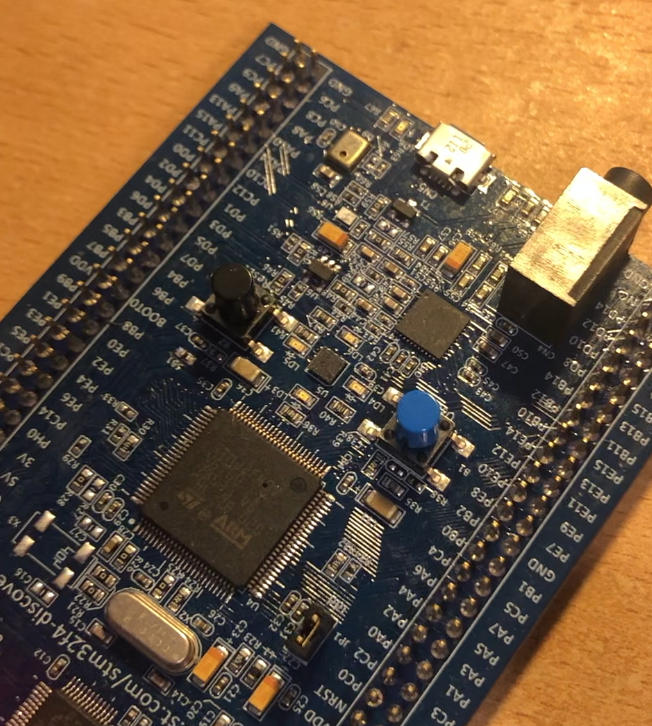
\includegraphics[width=\linewidth]{EventFlagsAus.jpg}
		\caption{suspendierte ISR}
		\label{fig:EventFlagAus}
	\end{subfigure}
	\hspace{1em}
	\begin{subfigure}{.250\textwidth}
		%		\centering
		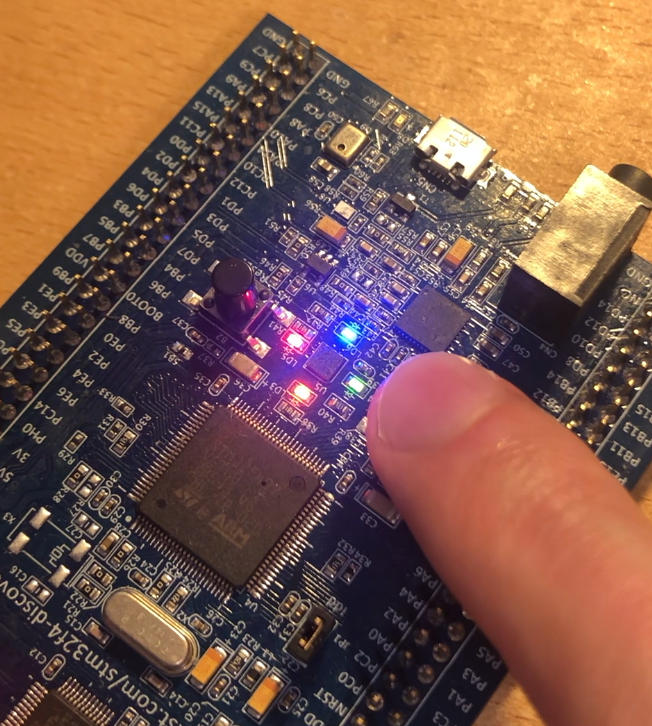
\includegraphics[width=\linewidth]{EventFlagsAn.jpg}
		\caption{aktive ISR}
		\label{fig:EventFlagAn}
	\end{subfigure}
	\caption{Beispiel von Event Flags für Interrupt-Management auf STM32F4 Discovery-Board}
	\label{fig:EventFlagBeispiel}
\end{figure}

Ereignisse können aperiodisch\todo{aperiodisch hat er mit Schwingungen zu tun. Eventuell anderes Wort für "nicht-periodisch" finden} und unvorhersehbar auftreten und - je nach Szenario - muss entsprechend schnell auf sie reagiert werden können, das entsprechende koordinierte Verhalten also möglichst synchron zum Zeitpunkt des Events ausgelöst werden. Um dies zu erreichen, wird eine \textbf{I}nterrupt \textbf{S}ervice \textbf{R}outine (ISR) eingesetzt, die auf das Eintreten eines Events wartet und - so lange keines eingetreten ist - sich in einem suspendierten Zustand befindet \autocite[vgl.][87]{Cooling2017}. Ein Beispiel für ein solches Ereignis kann ein Hardware-Interrupt sein wie er in Abbildung \ref{fig:EventFlagBeispiel} gezeigt wird: Erst mit gedrücktem bzw. gehaltenem blauen Button leuchten die vier LEDs auf (\ref{fig:EventFlagAn}).\\

Der schematische Ablauf mit Event Flags ist mit Abbildung \ref{fig:ConditionFlag} durchaus vergleichbar, nur dass jetzt Task A durch eine ISR ersetzt wird und eine Eingabe in Form des ausgelösten Ereignisses bekommt bevor das Event Flag gesetzt wird \autocite[vgl.][87]{Cooling2017}. Als weiterführende Lektüre zum Thema Interrupt und Interrupt Service Routine sei \autocite{MikrocontrollerInterrupt} oder weitere Fachliteratur empfohlen. Weiterhin spielt für die hier gewünschten Task-Synchronisierung der Zeitraum, in dem der Empfänger - hier Task B - das Event Flag überprüft eine größere und wichtigere Rolle: Für eine dynamische Reaktion auf ein Ereignis ist ein entsprechend kleines, periodisches Zeitfenster erforderlich. In der in Abbildung \ref{fig:EventFlagBeispiel} dargestellte Demonstration prüft Task B beispielsweise alle 500 Millisekunden ob das zugehörige Event Flag gesetzt ist. Ein weiter mit einer 2 Sekunden-Periode durchgeführter Versuch funktionierte ebenfalls, zeigte aber kein flüssiges Verhalten und kann für dieses Szenario ungeeignet sein. Um das Betriebsystem zu entlasten, wird Task B nach jeder negativen Überprüfung bis zur nächsten Iteration suspendiert, womit Ressourcen für andere Aufgaben frei werden.\\ 

Die Anwendung der unter \ref{subsec:Koordinierung_mit_Condition_Flags} vorgestellten Techniken zu Condition Flags (z.B. Flag Gruppen) sind auch auf das Konstrukt der Event Flags übertragbar. Somit ist sowohl eine verbesserte und sichere Implementierung bzw. auch eine für eine größere Anzahl Event Flags vorhanden.\\

Wie eingangs bereits erwähnt, funktioniert diese Synchronisierung lediglich in eine Richtung: Die Interrupt Service Routine wird durch das vordefinierte Event (Interrupt) geweckt und setzt das entsprechende Flag, welches vom Empfänger-Task registriert wird. Ist die Prüfungsperiode entsprechend den Anforderungen gewählt, wird eine angenäherte Synchronisierung von Ereignis und Reaktion bzw. ISR und Empfänger-Task erreicht. Sollen zwei Tasks synchronisiert werden, ist eine andere Methodik anzuwenden, die im nächsten Abschnitt vorgestellt wird.

\subsection{Task-Synchronisation über Signale}
\label{subsec:Task_Synchronisation_Signale}
Mit den bisher vorgestellten Techniken - Condition Flag und Event Flag - lässt sich bereits eine Koordination bzw. eine Einbahnstraßen-Synchronisation implementieren. Bei einer Problemstellung, bei der etwa mehrere Tasks nach und nach in eine Art Wartestellung gehen (etwa weil ihre Aufgabe erfüllt ist) und alle zu einem gleichen (synchronen) Zeitpunkt erneut starten sollen, helfen diese Konstrukte allerdings nicht weiter. Hierfür gibt es das Konzept der Signale.\\

Die in Tabelle \ref{tab:Konstrukte} angegebenen Operationen (\texttt{Wait}, \texttt{Send} und \texttt{Check}) lassen bereits einen anderen Umgang als bei Flags erahnen: Eine zentrale Stelle (diese kann sowohl das Betriebssystem selbst bereitstellen oder auch ein eigenes konzipiertes Objekt) übernimmt die Signalverwaltung. Bei ihr registrieren sich die beteiligten Tasks zunächst wenn eine der o.g. Operationen ausgeführt wird und diese übernimmt auch die Steuerung des Signals. Abbildung \ref{fig:Signale_gesamt} stellt die drei auftretenden Möglichkeiten vor.

\begin{figure}[h]
	\centering
	\fbox{
	\begin{subfigure}[t]{.39\columnwidth} % Werte mal so eingestellt lassen! .39
		\def\svgwidth{\columnwidth} % Breite wird auf Blattbreite (spalte) gesetzt
		\input{Signale_a.pdf_tex}
		\caption{\label{subfig:Signale_a}}
	\end{subfigure}
}\fbox{
	\begin{subfigure}[t]{.387\columnwidth} % Werte mal so eingestellt lassen! .387
		\def\svgwidth{\columnwidth}
		\input{Signale_b.pdf_tex}
		\caption{\label{subfig:Signale_b}}
	\end{subfigure}
}\fbox{
	\begin{subfigure}[t]{.1918\columnwidth} % Werte mal so eingestellt lassen! .1918
		\def\svgwidth{\columnwidth}
		\input{Signale_c.pdf_tex}
		\caption{\label{subfig:Signale_c}}
	\end{subfigure}
}
	\begin{subfigure}{.40\columnwidth} % Werte mal so eingestellt lassen! .40
		\def\svgwidth{\columnwidth}
		\input{Signale_Legende.pdf_tex}
	\end{subfigure}
	\caption{\label{fig:Signale_gesamt}Task-Synchronisation mittels Signalen \autocite[vgl.][90]{Cooling2017}}
\end{figure}

Zunächst sollen bei (a) und (b) zwei Tasks synchronisiert werden. Beide Darstellungen unterscheiden sich lediglich in der Reihenfolge, welche Operation zuerst auf ein Signal gewirkt wird: Der Task, welcher sich zuerst mit einer Operation meldet, wird suspendiert bis er zusammen mit dem anderen Task das synchronisierte Signal zur Wiederaufnahme erhält. Beide starten dann synchron.
Option (c) zeigt, wie ein einzelner Task synchronisiert wird, ohne bekanntes Mitspiel anderer Tasks: Eine Überprüfung des Signals erfolgt und ggf. eine Suspendierung oder eine sofortige Wiederaufnahme. Hierbei kann das Signal (Exekutive) auch eine interne Logik besitzen und zum Timing verschiedener einzelner oder mehrerer Tasks benutzt werden.\\

Die Umsetzung von Signalen erfolgt meist über Funktionen, wie im folgenden mit C beispielhaft demonstriert:
\begin{lstlisting}[language=C]
void Send(SyncSignal SignalName);
void Wait(SyncSignal SignalName);

typedef enum {false, true} bool;
bool Check(SyncSignal SignalName);
\end{lstlisting}
Diese Technik synchronisiert - anders als Event Flags - in beide Richtungen.

\section{Datentransfer ohne Synchronisation oder Koordination}
Ist ein Datenaustausch zwischen Tasks erforderlich, aber nicht an Koordinierungs- und Synchronisationskriterien gebunden, unterliegt also weder einer zeitlichen Vorgabe noch einem Ablauf, werden verschiedene Datenstrukturen zum Austausch zwischen Tasks verwendet.  
\subsection{Überblick}
\subsection{Pools}
\subsection{Queues}
\section{Task-Synchronisation mit Datentransfer}
Daten, die mit einer zeitlichen Priorität zwischen Tasks ausgetauscht werden, also genau zum richtigen Zeitpunkt beim Empfänger bereit stehen müssen, werden ebenfalls mit einer Datenstruktur transferiert. An diese besteht jedoch ein höherer Anspruch, da sie die Synchronisation sicherstellen muss.
\subsection{Mailbox}
\section{Zusammenfassung}

\printbibliography


\end{document}